\documentclass[a4paper, 11pt]{article}\usepackage[]{graphicx}\usepackage[]{color}
%% maxwidth is the original width if it is less than linewidth
%% otherwise use linewidth (to make sure the graphics do not exceed the margin)
\makeatletter
\def\maxwidth{ %
  \ifdim\Gin@nat@width>\linewidth
    \linewidth
  \else
    \Gin@nat@width
  \fi
}
\makeatother

\definecolor{fgcolor}{rgb}{0.345, 0.345, 0.345}
\newcommand{\hlnum}[1]{\textcolor[rgb]{0.686,0.059,0.569}{#1}}%
\newcommand{\hlstr}[1]{\textcolor[rgb]{0.192,0.494,0.8}{#1}}%
\newcommand{\hlcom}[1]{\textcolor[rgb]{0.678,0.584,0.686}{\textit{#1}}}%
\newcommand{\hlopt}[1]{\textcolor[rgb]{0,0,0}{#1}}%
\newcommand{\hlstd}[1]{\textcolor[rgb]{0.345,0.345,0.345}{#1}}%
\newcommand{\hlkwa}[1]{\textcolor[rgb]{0.161,0.373,0.58}{\textbf{#1}}}%
\newcommand{\hlkwb}[1]{\textcolor[rgb]{0.69,0.353,0.396}{#1}}%
\newcommand{\hlkwc}[1]{\textcolor[rgb]{0.333,0.667,0.333}{#1}}%
\newcommand{\hlkwd}[1]{\textcolor[rgb]{0.737,0.353,0.396}{\textbf{#1}}}%

\usepackage{framed}
\makeatletter
\newenvironment{kframe}{%
 \def\at@end@of@kframe{}%
 \ifinner\ifhmode%
  \def\at@end@of@kframe{\end{minipage}}%
  \begin{minipage}{\columnwidth}%
 \fi\fi%
 \def\FrameCommand##1{\hskip\@totalleftmargin \hskip-\fboxsep
 \colorbox{shadecolor}{##1}\hskip-\fboxsep
     % There is no \\@totalrightmargin, so:
     \hskip-\linewidth \hskip-\@totalleftmargin \hskip\columnwidth}%
 \MakeFramed {\advance\hsize-\width
   \@totalleftmargin\z@ \linewidth\hsize
   \@setminipage}}%
 {\par\unskip\endMakeFramed%
 \at@end@of@kframe}
\makeatother

\definecolor{shadecolor}{rgb}{.97, .97, .97}
\definecolor{messagecolor}{rgb}{0, 0, 0}
\definecolor{warningcolor}{rgb}{1, 0, 1}
\definecolor{errorcolor}{rgb}{1, 0, 0}
\newenvironment{knitrout}{}{} % an empty environment to be redefined in TeX

\usepackage{alltt}
\usepackage{covington}
\usepackage{amssymb}
\usepackage{amsmath}
\usepackage[catalan]{babel}
\usepackage{graphicx}
\usepackage{eurosym}
\textheight=23.94cm 
\textwidth=17cm 
\topmargin=-1cm 
\oddsidemargin=-0.5cm 
 
\newcommand{\header}[4]{
	\begin{center}
		\rule{\linewidth}{0.5pt}
		
		{\small{#1}}
      
        \vspace{0.2in}
        
		{\large{#2}}
		
        \vspace{0.2in}
        
		{\small{#3}}
		
		\vspace{0.15in}
		
		{#4}
		
		\vspace{-0.1in}
		\rule{\linewidth}{0.6pt}
	\end{center}
}
\IfFileExists{upquote.sty}{\usepackage{upquote}}{}
\begin{document}
 
\header{\sc Barcelona Graduate School of Economics \hfill Master's Degree in Data Science}{\bf Statistical Modeling and Inference $-$ Problem Set \#2}{\sc Niti Mishra $\cdot$ Miquel Torrens $\cdot$ B\'alint V\'an}{October 18\textsuperscript{th}, 2015}
Solution to proposed exercises.\\
% PROBLEM SET 2 (PART 1)
% EXERCISE 1
\newline \textbf{\underline{Exercise 1}}\\
\newline We need to solve:
\begin{eqnarray}
\max_{\mathbf{w}} -2 \log p(\mathbf{w | t, X}) &=&  -2q \mathbf{t}^T \mathbf{\Phi w} + q \mathbf{w}^T \mathbf{\Phi}^T \mathbf{\Phi w} + (\mathbf{w - \mu})^T \mathbf{D} (\mathbf{w - \mu}) + C \nonumber \\
&=&  -2q \mathbf{t}^T \mathbf{\Phi w} + q \mathbf{w}^T \mathbf{\Phi}^T \mathbf{\Phi w} + \mathbf{w}^T \mathbf{D w} - 2 \mathbf{w}^T \mathbf{D} \mathbf{\mu} + \mathbf{\mu}^T \mathbf{D \mu} + C \nonumber
\end{eqnarray}
The term $C$ includes all constant terms not dependant on $\mathbf{w}$. Now we maximize with respect to $\mathbf{w}$ and set to zero:
\begin{eqnarray}
-2q \mathbf{t}^T \mathbf{\Phi} + q \mathbf{w}^T \left(\mathbf{\Phi}^T \mathbf{\Phi} + \left( \mathbf{\Phi}^T \mathbf{\Phi} \right)^T \right) + \mathbf{w}^T \left( \mathbf{D} + \mathbf{D}^T \right) - 2 \left( \mathbf{D} \mathbf{\mu} \right)^T = 0 \nonumber
\end{eqnarray}
During the derivation we will recurrently use two properties: $\mathbf{D} = \mathbf{D}^T$, as it is symmetric by construction, and $\left( \mathbf{\Phi}^T \mathbf{\Phi} \right)^T = \mathbf{\Phi}^T \mathbf{\Phi}$, which is a straightforward calculation. We just need to rearrange terms to reach the normal equations:
\begin{eqnarray}
2 \mathbf{w}^T\mathbf{D} -2 \mathbf{\mu}^T \mathbf{D}^T -2 q \mathbf{t}^T \mathbf{\Phi} + 2q\mathbf{w}^T \mathbf{\Phi}^T \mathbf{\Phi} &=& 0 \nonumber \\
\mathbf{w}^T \left( \mathbf{D} + q \mathbf{\Phi}^T \mathbf{\Phi} \right) &=& q\mathbf{t}^T \mathbf{\Phi} + \left( \mathbf{D\mu} \right)^T  \nonumber \\
\left( \mathbf{D} + q \mathbf{\Phi}^T \mathbf{\Phi} \right)^T \mathbf{w} &=& q\mathbf{\Phi}^T \mathbf{t} + \left( \mathbf{D\mu} \right) \nonumber
\end{eqnarray}
To finally obtain the normal equations:
\begin{eqnarray}
\left( \mathbf{D} + q \mathbf{\Phi}^T \mathbf{\Phi} \right) \mathbf{w} = q\mathbf{\Phi}^T \mathbf{t} + \mathbf{D\mu} \nonumber
\end{eqnarray}
Hence proved.\\
% EXERCISE 2
\newpage
\textbf{\underline{Exercise 2}}\\
\newline \underline{Part 1}. Plotting the data:\\
\begin{center}
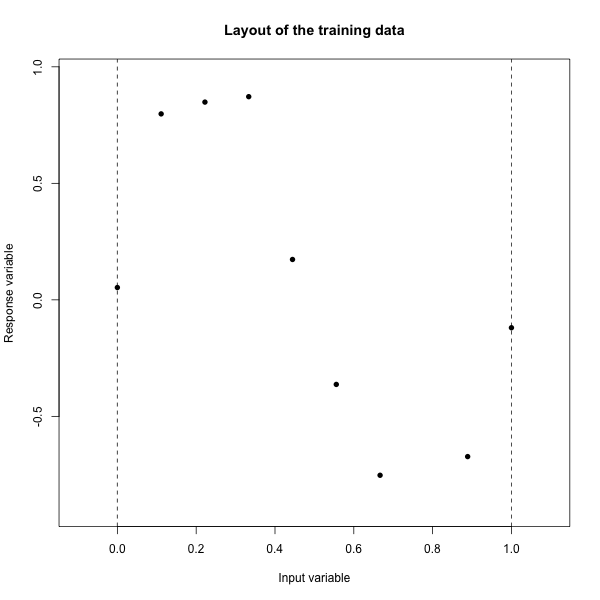
\includegraphics[scale=0.6]{ps2_plot1.png}
\end{center}
\underline{Part 2}. The \texttt{phix} function:
\begin{knitrout}\small
\definecolor{shadecolor}{rgb}{0.969, 0.969, 0.969}\color{fgcolor}\begin{kframe}
\begin{alltt}
\hlcom{################################################################################}
\hlcom{# Function "phix"}
\hlstd{phix} \hlkwb{<-} \hlkwa{function}\hlstd{(}\hlkwc{x}\hlstd{,} \hlkwc{M}\hlstd{,} \hlkwc{basis}\hlstd{) \{}
\hlcom{################################################################################}
  \hlcom{# Check correctness of input x}
  \hlkwa{if} \hlstd{(x} \hlopt{<} \hlnum{0} \hlopt{||} \hlstd{x} \hlopt{>} \hlnum{1}\hlstd{) \{}
    \hlkwd{stop}\hlstd{(}\hlstr{'out-of-range values in the input vector "x".'}\hlstd{)}
  \hlstd{\}}

  \hlcom{# Perform the calculations  }
  \hlkwa{if} \hlstd{(basis} \hlopt{==} \hlstr{'poly'}\hlstd{) \{}
    \hlstd{out} \hlkwb{<-} \hlkwd{rep}\hlstd{(}\hlnum{NA}\hlstd{,} \hlkwc{length} \hlstd{= M} \hlopt{+} \hlnum{1}\hlstd{)}
    \hlkwd{sapply}\hlstd{(}\hlkwd{c}\hlstd{(}\hlnum{0}\hlstd{,} \hlnum{1}\hlopt{:}\hlstd{M),} \hlkwa{function}\hlstd{(}\hlkwc{i}\hlstd{) \{}
      \hlstd{out[i} \hlopt{+} \hlnum{1}\hlstd{]} \hlkwb{<<-} \hlstd{x}\hlopt{^}\hlstd{i}
    \hlstd{\})}
  \hlstd{\}} \hlkwa{else if} \hlstd{(basis} \hlopt{==} \hlstr{'Gauss'}\hlstd{) \{}
    \hlcom{#mus <- seq(0, 1, M ** (-1))}
    \hlstd{mus} \hlkwb{<-} \hlkwd{seq}\hlstd{(}\hlnum{0}\hlstd{,} \hlnum{1}\hlstd{,} \hlkwc{length.out} \hlstd{= M)}
    \hlstd{out} \hlkwb{<-} \hlkwd{rep}\hlstd{(}\hlnum{NA}\hlstd{,} \hlkwc{length} \hlstd{= M)}
    \hlkwd{sapply}\hlstd{(}\hlnum{1}\hlopt{:}\hlstd{M,} \hlkwa{function}\hlstd{(}\hlkwc{i}\hlstd{) \{}
      \hlstd{out[i]} \hlkwb{<<-} \hlkwd{exp}\hlstd{((}\hlopt{-}\hlstd{(x} \hlopt{-} \hlstd{mus[i])} \hlopt{**} \hlnum{2}\hlstd{)} \hlopt{/} \hlnum{0.1}\hlstd{)}
    \hlstd{\})}
    \hlstd{out} \hlkwb{<-} \hlkwd{c}\hlstd{(}\hlnum{1}\hlstd{, out)}
  \hlstd{\}} \hlkwa{else} \hlstd{\{}
    \hlkwd{stop}\hlstd{(}\hlstr{'specify a valid option for the parameter "basis".'}\hlstd{)}
  \hlstd{\}}

  \hlcom{# Return the values}
  \hlkwd{return}\hlstd{(out)}
\hlstd{\}}
\end{alltt}
\end{kframe}
\end{knitrout}
\underline{Part 3}. The \texttt{post.params} function:
\begin{knitrout}\small
\definecolor{shadecolor}{rgb}{0.969, 0.969, 0.969}\color{fgcolor}\begin{kframe}
\begin{alltt}
\hlcom{################################################################################}
\hlcom{# Function "post.params"}
\hlstd{post.params} \hlkwb{<-} \hlkwa{function}\hlstd{(}\hlkwc{tdata}\hlstd{,} \hlkwc{M}\hlstd{,} \hlkwc{basis}\hlstd{,} \hlkwc{phix}\hlstd{,} \hlkwc{delta}\hlstd{,} \hlkwc{q}\hlstd{) \{}
\hlcom{################################################################################}
  \hlcom{# Input data}
  \hlstd{t} \hlkwb{<-} \hlstd{tdata[,} \hlstr{'t'}\hlstd{]}  \hlcom{# Response variable}
  \hlstd{x} \hlkwb{<-} \hlstd{tdata[,} \hlstr{'x'}\hlstd{]}  \hlcom{# Input variable}

  \hlcom{# Initialize Phi matrix}
  \hlstd{phi} \hlkwb{<-} \hlkwd{matrix}\hlstd{(}\hlkwc{nrow} \hlstd{=} \hlkwd{length}\hlstd{(x),} \hlkwc{ncol} \hlstd{= M} \hlopt{+} \hlnum{1}\hlstd{)}
  \hlkwd{sapply}\hlstd{(}\hlnum{1}\hlopt{:}\hlkwd{length}\hlstd{(x),} \hlkwa{function}\hlstd{(}\hlkwc{i}\hlstd{) \{}
    \hlstd{phi[i, ]} \hlkwb{<<-} \hlkwd{phix}\hlstd{(}\hlkwc{x} \hlstd{= x[i],} \hlkwc{M} \hlstd{= M,} \hlkwc{basis} \hlstd{= basis)}
  \hlstd{\})}

  \hlcom{# Function parameter}
  \hlstd{lambda} \hlkwb{<-} \hlstd{delta} \hlopt{/} \hlstd{q}

  \hlstd{Q} \hlkwb{<-} \hlstd{delta} \hlopt{*} \hlkwd{diag}\hlstd{(}\hlkwd{ncol}\hlstd{(phi))} \hlopt{+} \hlstd{q} \hlopt{*} \hlkwd{t}\hlstd{(phi)} \hlopt \hlstd{phi}
  \hlstd{w.bayes} \hlkwb{<-} \hlstd{q} \hlopt{*} \hlkwd{solve}\hlstd{(Q)} \hlopt \hlkwd{t}\hlstd{(phi)} \hlopt \hlstd{t}

  \hlcom{# Results}
  \hlkwd{return}\hlstd{(}\hlkwd{list}\hlstd{(}\hlkwc{w.bayes} \hlstd{= w.bayes,} \hlkwc{Q} \hlstd{= Q))}
\hlstd{\}}
\end{alltt}
\end{kframe}
\end{knitrout}
\underline{Part 4}. Plotting the estimated linear predictor:
\begin{center}
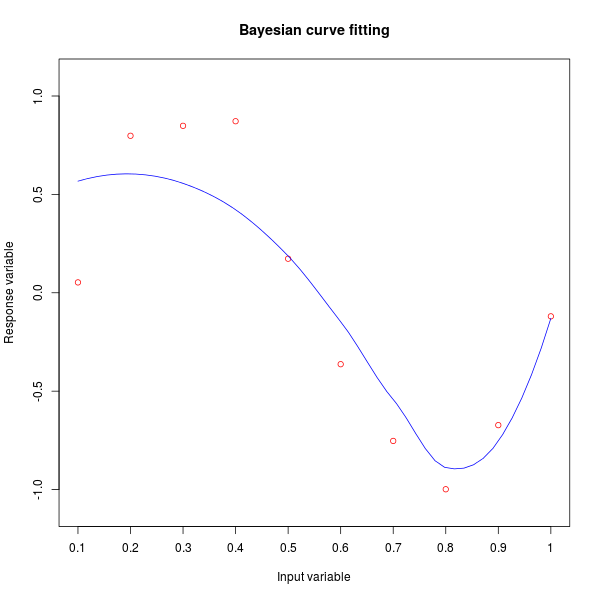
\includegraphics[scale = 0.5]{ps2_plot2.png}
\end{center}
% PROBLEM SET 2 (PART 2)
% EXERCISE 3
\newpage
\textbf{\underline{Exercise 3}}\\
\underline{Part 1}. The function that returns the mean and the precision of the predictive distribution at each of the inputs:
\begin{knitrout}\small
\definecolor{shadecolor}{rgb}{0.969, 0.969, 0.969}\color{fgcolor}\begin{kframe}
\begin{alltt}
\hlcom{################################################################################}
\hlstd{bayesian.precision} \hlkwb{<-} \hlkwa{function}\hlstd{(}\hlkwc{x}\hlstd{) \{}
\hlcom{################################################################################}
  \hlcom{# Parameters}
  \hlstd{M} \hlkwb{<-} \hlnum{9}
  \hlstd{delta} \hlkwb{<-} \hlnum{1L}
  \hlstd{q} \hlkwb{<-} \hlnum{0.1} \hlopt{**} \hlstd{(}\hlopt{-}\hlnum{2}\hlstd{)}

  \hlcom{# Initialize Phi matrix (THINK post.params)}
  \hlstd{phi} \hlkwb{<-} \hlkwd{matrix}\hlstd{(}\hlkwc{nrow} \hlstd{=} \hlkwd{length}\hlstd{(x),} \hlkwc{ncol} \hlstd{= M} \hlopt{+} \hlnum{1}\hlstd{)}
  \hlkwd{sapply}\hlstd{(}\hlnum{1}\hlopt{:}\hlkwd{length}\hlstd{(x),} \hlkwa{function}\hlstd{(}\hlkwc{i}\hlstd{) \{}
    \hlstd{phi[i, ]} \hlkwb{<<-} \hlkwd{phix}\hlstd{(}\hlkwc{x} \hlstd{= x[i],} \hlkwc{M} \hlstd{=} \hlnum{9}\hlstd{,} \hlkwc{basis} \hlstd{=} \hlstr{'Gauss'}\hlstd{)}
  \hlstd{\})}

  \hlcom{# Execute the function with the specified parameters}
  \hlstd{params} \hlkwb{<-} \hlkwd{post.params}\hlstd{(cd,} \hlkwc{M} \hlstd{=} \hlnum{9}\hlstd{,} \hlkwc{basis} \hlstd{=} \hlstr{'Gauss'}\hlstd{, phix,}
                         \hlkwc{delta} \hlstd{=} \hlnum{1L}\hlstd{,} \hlkwc{q} \hlstd{=} \hlnum{0.1} \hlopt{**} \hlstd{(}\hlopt{-}\hlnum{2}\hlstd{))}

  \hlcom{# Resulting parameters}
  \hlstd{Q} \hlkwb{<-} \hlstd{params[[}\hlnum{2}\hlstd{]]}
  \hlstd{w.bayes} \hlkwb{<-} \hlstd{params[[}\hlnum{1}\hlstd{]]}

  \hlcom{# Predicted values}
  \hlstd{means} \hlkwb{<-} \hlstd{phi} \hlopt \hlstd{w.bayes}
  \hlstd{vars} \hlkwb{<-} \hlstd{phi} \hlopt \hlkwd{solve}\hlstd{(Q)} \hlopt \hlkwd{t}\hlstd{(phi)} \hlopt{+} \hlstd{q} \hlopt{**} \hlstd{(}\hlopt{-}\hlnum{1}\hlstd{)}

  \hlcom{# Return}
  \hlkwd{return}\hlstd{(}\hlkwd{list}\hlstd{(}\hlkwc{means} \hlstd{= means,} \hlkwc{vars} \hlstd{=} \hlkwd{diag}\hlstd{(vars)))}
\hlstd{\}}
\end{alltt}
\end{kframe}
\end{knitrout}
\underline{Part 2}. Plotting the predicted mean with its standard predictive posterior deviation:
\begin{center}
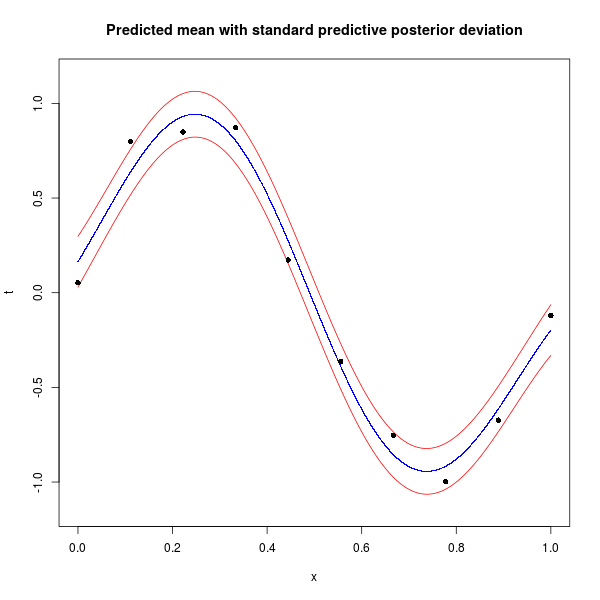
\includegraphics[scale=0.6]{ps2_plot3.png}
\end{center}
\underline{Part 3}. Replicating the plot of the slides:
\begin{center}
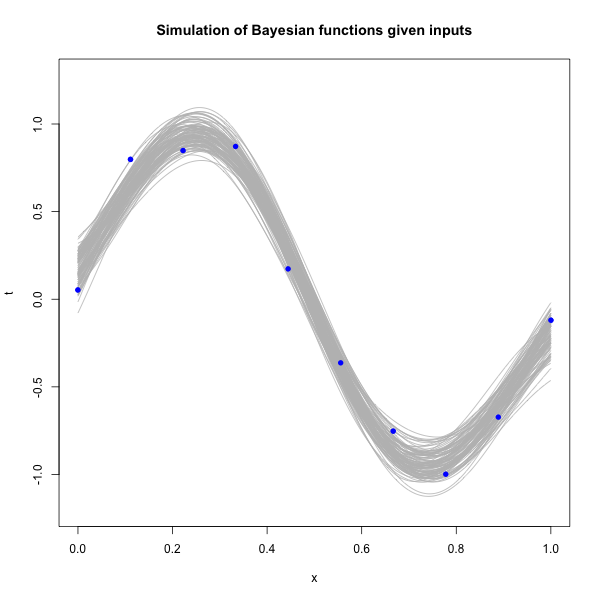
\includegraphics[scale=0.6]{ps2_plot4.png}
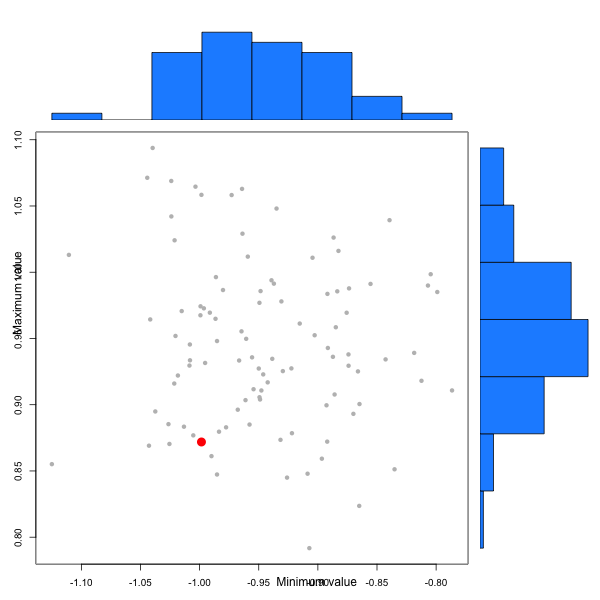
\includegraphics[scale=0.5]{ps2_plot5.png}
\end{center}
% EXERCISE 4
\newpage
\textbf{\underline{Exercise 4}}\\

\end{document}
